\subsubsection{Language model architectures}
\label{subsubsec:language_model_architectures}

\subsubsection{Masked language models}

Masked language models only used an encoder, not a decoder.
The first encoder takes as input the sequence of embeddings with
positional encodings. The subsequent encoders take as input the output of the previous encoder.
The output of the last encoder is called the \textbf{contextualized embeddings} of dimension $k$.
At this point the \textbf{contextualized embeddings} depend on the entire input sequence.
Each contextualized embedding is then passed through a \textbf{classification head}
that outputs a probability distribution for that token.
The most famous masked language model is BERT (Bidirectional Encoder Representations from Transformers).
BERT-Base has 12 attention heads and 12 encoders, $k=768$.
BERT-Large has 24 attention heads and 24 encoders, $k=1024$.
Bert has been trained with 2 objectives:
\begin{itemize}
    \item \textbf{Prediction of the masked token}
    \item \textbf{NSP (Next Sentence Prediction)}
\end{itemize}
The tokenizer used is called \textbf{WordPiece}.
In general, the input is composed of two sentences, the model has to predict if the second sentence
comes after or before the first sentence.
The input is composed like this:
\begin{itemize}
    \item [CLS]
    \item Sentence 1
    \item [SEP]
    \item Sentence 2
    \item [SEP]
    \item Padding
\end{itemize}
We also have a sentence token called $S_i$ that is summed to the embeddings in the sentences.
If $w_i$ is in the first sentence $S_1$ is used, if $w_i$ is in the second sentence $S_2$ is used.
Then a classification head is used to predict if the second sentence comes after or before the first sentence,
the classification head takes as input the [CLS] contextualized embedding.

The dataset is generated by an algorithm that takes as input a sentence and outputs a \textbf{masked} sentence.
Most of the output sentence is the same as the input sentence, we also return the indices of the masked tokens $I_s$.
15\% of the tokens are masked. A masked token can be:
\begin{itemize}
    \item Replaced with the [MASK] token $0.8$
    \item Replaced with a random token $0.1$
    \item Leave the token as it is $0.1$
\end{itemize}
In this way the model also sees a small portion of the data unmasked. The random token is used to handle also
typos in the input data.

The loss for the masked language model task is:
\[
    \mathcal{L}_MLM=\sum_{s\in D}\sum_{i\in I_s}-\log P[w_i|\tilde{s}]
\]

For the NSP task the dataset is generated by taking the original dataset and for each sentence
we randomly select the previous or the next sentence. The target is 0 if the sentence comes before
and 1 if the sentence comes after. The new dataset is called $D'$
The loss for the NSP task is:
\[
    \mathcal{L}_NSP=\sum_{s\in D'}-\log P[c|\text{[cls]}s_1\text{[sep]}s_2\text{[sep]}]
\]
where $P[c]$ is the probability of the target class.

The total loss is $\mathcal{L}=\mathcal{L}_MLM+\mathcal{L}_NSP$.
The [CLS] contextualized embedding is assumed to be the embedding of the whole document.

To use [CLS] as a representation of the document we need to fine-tune the model on a specific dataset.
To fine-tune bert for ranking documents we can use the ordering binary classification capabilities on bert.

\begin{figure}[H]
    \centering
    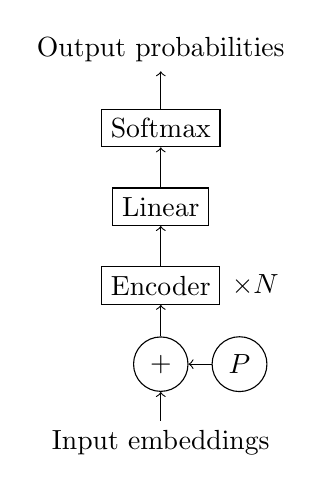
\begin{tikzpicture}
        % Nodes
        \node (input) {Input embeddings};
        \node (pos_sum) [draw, circle, above of=input] {$+$};
        \node (pos) [draw, circle, right of=pos_sum] {$P$};
        \node (encoder) [draw, rectangle, above of=pos_sum] {Encoder};
        \node (encoder_count) [right of=encoder, node distance=1.2cm] {$\times N$};
        \node (linear) [draw, rectangle, above of=encoder] {Linear};
        \node (softmax) [draw, rectangle, above of=linear] {Softmax};
        \node (output) [above of=softmax] {Output probabilities};

        % Arrows
        \draw [->] (input) -- (pos_sum);
        \draw [->] (pos) -- (pos_sum);
        \draw [->] (pos_sum) -- (encoder);
        \draw [->] (encoder) -- (linear);
        \draw [->] (linear) -- (softmax);
        \draw [->] (softmax) -- (output);

    \end{tikzpicture}
    \caption{Masked language model architecture}
    \label{fig:masked_language_model_architecture}
\end{figure}

\subsubsection{Causal language models}

In causal language models, we only have a decoder.
How can we only use the decoder if it needs another input $E$?
We cut the $E$ input, we only use the MHCA and remove the MHA and the second layer normalization.
We call this a \textbf{simple decoder}.

After a sequence of simple decoders, we add a classification head that outputs the probability of the
next token. The loss is the cross-entropy loss.

To use the model, we just pass in the input sequence, get the last next token probability, generate the next
token, add it to the input sequence and repeat the process. The process of generating the next token
and appending it to the input sequence is called \textbf{autoregressive generation}.

\begin{figure}[H]
    \centering
    \begin{tikzpicture}
        % Nodes
        \node (input) {Output embeddings (shifted right)};
        \node (pos_sum) [draw, circle, above of=input] {$+$};
        \node (pos) [draw, circle, right of=pos_sum] {$P$};
        \node (mhca) [draw, rectangle, above of=pos_sum, node distance=1.5cm] {MHCA};
        \node (sum) [draw, circle, above of=mhca] {$+$};
        \node (layer_norm) [draw, rectangle, above of=sum] {LayerNorm};
        \node (linear) [draw, rectangle, above of=layer_norm] {Linear};
        \node (softmax) [draw, rectangle, above of=linear] {Softmax};
        \node (output) [above of=softmax] {Output probabilities};

        % Arrows
        \draw [->] (input) -- (pos_sum);
        \draw [->] (pos) -- (pos_sum);
        \draw [->] (pos_sum) -- (mhca);
        \draw [->] (pos_sum) -- ++(0,0.9) -| ($(mhca.south) + (0.2,0)$);
        \draw [->] (pos_sum) -- ++(0,0.9) -| ($(mhca.south) + (-0.2,0)$);
        \draw [->] (pos_sum) -- ++(0,0.7) -- ++(1,0) |- (sum);
        \draw [->] (mhca) -- (sum);
        \draw [->] (sum) -- (layer_norm);
        \draw [->] (layer_norm) -- (linear);
        \draw [->] (linear) -- (softmax);
        \draw [->] (softmax) -- (output);
        \draw [->, dashed] (output.east) -- ++(2,0) -- ++(0,-3) node[above, rotate=270] {Last token} |- (input.east); 

        \draw [dashed] ($(mhca) - (1.5,1)$) rectangle ($(layer_norm) + (1.5,0.5)$);
        \node at ($(layer_norm) + (-2,1)$) {Simple decoder};
        \node at ($(layer_norm) + (-2,-1.2)$) {$N\times$};
    \end{tikzpicture}
    \caption{Causal language model architecture}
    \label{fig:causal_language_model_architecture}
\end{figure}

The most famous causal language model is GPT (Generalized Pre-trained Transformer).
For the new versions most of the parameters are not disclosed.
\begin{tabular}{|c|c|c|c|c|c|c|}
    \hline
    Model & Layers & Heads & Embedding & Context & Params & Corpus \\
    \hline
    GPT-1 & 12 & 12 & 768 & 512 & 117M & 4.5GB \\
    GPT-2 & 48 & 12 & 1600 & 1024 & 1.5B & 40GB \\
    GPT-3 & 96 & 12 & 12288 & 2048 & 175B & 570GB \\
    \hline
    
\end{tabular}

Empirically has been shown that the larger the model, the larger the corpus, the better.
These empirical laws are called \textbf{scaling laws}.

Although rumors claim that the loss has plateaued (at the time of writing, we hope to find this out this month).

When we provide a model, at inference time, a prompt, the model will use the prompt as a kind of extra "parameter".
We call this behaviour \textbf{in-context learning}. The prompt can help in generating the output data.
The act of crafting a good prompt is called \textbf{prompt engineering}.

We are trying to create a template that we can then fill with some input data.
Given a template, we can generate a filled template and give it to the model.
The model will the use the information in the template and the information learned during training
to generate the output data.

A template can be seen as instructions for the task we want to perform.

We can also provide some demonstrations, examples of the task we want to perform.

If we prompt the model with just instructions, this is called \textbf{zero-shot}.
If we prompt both with instructions and demonstrations, this is called \textbf{few-shot}.

In providing a prompt, we exploit the fact that the input conditions all the subsequent tokens.
We have no certainty on the output, when the model generates content that is factually false
we call this \textbf{hallucination}.
The output can also contain \textbf{toxic content}.
The first approach used to mitigate these problems was to use further \textbf{fine-tuning}.

How can we fine-tune an LLM?
\begin{itemize}
    \item \textbf{Instruction fine-tuning}: we provide the model with instructions, some call this 
    "supervised" fine tuning even if it's obviously supervised like the rest of the training.
    This is very expensive. With \textbf{parameter efficient fine-tuning} to avoid being judged as "destroyer of the future of mankind"
    we can use some techniques to fine-tune the model with less data. \textbf{Low Rank Adaptation} is a 
    technique that freezes the model and train a second smaller model, the outputs of the second model
    are summed to the outputs of the first model. The second model learns the changes to the first model.
    The additional model is a simple matrix multiplication but with a big matrix, usually the matrix is
    decomposed in two smaller matrices.
    \item \textbf{Reinforcement learning with human feedback (RLHF)}: we want to tell a model which outputs are good and which are bad.
    We need to provide the model a human feedback about its outputs. This technique was used to fine-tune GPT-3.5
    into ChatGPT.
\end{itemize}
